\documentclass[8pt,aspectratio=169]{beamer}
\usetheme{Madrid}
\usepackage{graphicx}
\usepackage{booktabs}
\usepackage{adjustbox}
\usepackage{multicol}
\usepackage{amsmath}
\usepackage{amssymb}
\usepackage{tikz}
\usetikzlibrary{arrows.meta,positioning,shapes.callouts,shapes.geometric,decorations.pathreplacing}
\usepackage{colortbl}
\usepackage{pgfplots}
\pgfplotsset{compat=1.18}
\usepackage{hyperref}
\usepackage{algorithm}
\usepackage{algorithmic}

% Color definitions
\definecolor{mlblue}{RGB}{0,102,204}
\definecolor{mlpurple}{RGB}{51,51,178}
\definecolor{mllavender}{RGB}{173,173,224}
\definecolor{mllavender2}{RGB}{193,193,232}
\definecolor{mllavender3}{RGB}{204,204,235}
\definecolor{mllavender4}{RGB}{214,214,239}
\definecolor{mlorange}{RGB}{255, 127, 14}
\definecolor{mlgreen}{RGB}{44, 160, 44}
\definecolor{mlred}{RGB}{214, 39, 40}
\definecolor{mlgray}{RGB}{127, 127, 127}

% Additional colors for template compatibility
\definecolor{lightgray}{RGB}{240, 240, 240}
\definecolor{midgray}{RGB}{180, 180, 180}
\definecolor{dfteal}{RGB}{0,128,128}
\definecolor{dfred}{RGB}{180,30,30}

% Backward compatibility: uppercase color names
\colorlet{MLPurple}{mlpurple}
\colorlet{MLBlue}{mlblue}
\colorlet{MLOrange}{mlorange}
\colorlet{MLGreen}{mlgreen}
\colorlet{MLRed}{mlred}
\colorlet{MLLavender}{mllavender}
\colorlet{MLGray}{mlgray}

% Apply custom colors to Madrid theme
\setbeamercolor{palette primary}{bg=mllavender3,fg=mlpurple}
\setbeamercolor{palette secondary}{bg=mllavender2,fg=mlpurple}
\setbeamercolor{palette tertiary}{bg=mllavender,fg=white}
\setbeamercolor{palette quaternary}{bg=mlpurple,fg=white}

\setbeamercolor{structure}{fg=mlpurple}
\setbeamercolor{section in toc}{fg=mlpurple}
\setbeamercolor{subsection in toc}{fg=mlblue}
\setbeamercolor{title}{fg=mlpurple}
\setbeamercolor{frametitle}{fg=mlpurple,bg=mllavender3}
\setbeamercolor{block title}{bg=mllavender2,fg=mlpurple}
\setbeamercolor{block body}{bg=mllavender4,fg=black}

% Remove navigation symbols
\setbeamertemplate{navigation symbols}{}

% Clean itemize/enumerate
\setbeamertemplate{itemize items}[circle]
\setbeamertemplate{enumerate items}[default]

% Reduce margins for more content space
\setbeamersize{text margin left=5mm,text margin right=5mm}

% Custom course footer
\setbeamertemplate{footline}{
  \leavevmode%
  \hbox{%
    \begin{beamercolorbox}[wd=.333333\paperwidth,ht=2.25ex,dp=1ex,center]{author in head/foot}%
      \usebeamerfont{author in head/foot}Methods and Algorithms
    \end{beamercolorbox}%
    \begin{beamercolorbox}[wd=.333333\paperwidth,ht=2.25ex,dp=1ex,center]{title in head/foot}%
      \usebeamerfont{title in head/foot}MSc Data Science
    \end{beamercolorbox}%
    \begin{beamercolorbox}[wd=.333333\paperwidth,ht=2.25ex,dp=1ex,right]{date in head/foot}%
      \usebeamerfont{date in head/foot}\insertframenumber{} / \inserttotalframenumber\hspace*{2ex}
    \end{beamercolorbox}}%
  \vskip0pt%
}

% Command for bottom annotation (Madrid-style)
\newcommand{\bottomnote}[1]{%
\vfill
\vspace{-2mm}
\textcolor{mllavender2}{\rule{\textwidth}{0.4pt}}
\vspace{1mm}
\footnotesize
\textbf{#1}
}

% Custom commands for course compatibility
\newcommand{\highlight}[1]{\textcolor{mlorange}{\textbf{#1}}}
\newcommand{\mathbold}[1]{\boldsymbol{#1}}

% Compact list environment
\newenvironment{compactlist}{%
  \begin{itemize}%
    \setlength{\itemsep}{2pt}%
    \setlength{\parskip}{0pt}%
    \setlength{\parsep}{0pt}%
}{%
  \end{itemize}%
}

\title[L06b: Reinforcement Learning]{Reinforcement Learning: A Visual Guide}
\subtitle{Teaching Computers to Make Decisions}
\author{Prof.\ Dr.\ J\"org Osterrieder}
\institute{Methods and Algorithms --- MSc Data Science}
\date{Spring 2026}

\begin{document}

% Slide 1: Title Page
\begin{frame}[plain]
\titlepage
\end{frame}

% Slide 2: XKCD Opening
\begin{frame}{How Do You Teach a Computer to Decide?}
\begin{columns}[c]
\begin{column}{0.45\textwidth}
\centering
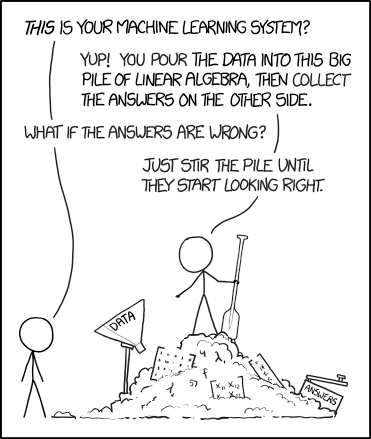
\includegraphics[height=0.55\textheight]{images/1838_machine_learning.png}
\end{column}
\begin{column}{0.50\textwidth}
\large
\textit{How do you teach a computer to \textbf{make good decisions} without a teacher?}

\vspace{6mm}
Today: \textbf{Reinforcement Learning} --- learning by trial and error.
\end{column}
\end{columns}
\bottomnote{XKCD \#1838 by Randall Munroe (CC BY-NC 2.5)}
\end{frame}

% Slide 3: Learning Objectives
\begin{frame}{What You Will Learn Today}
\begin{enumerate}
\setlength{\itemsep}{8pt}
\item \textbf{Describe the RL agent-environment loop}
\item \textbf{Explain the explore vs exploit tradeoff}
\item \textbf{Identify when RL applies} to real problems
\end{enumerate}
\bottomnote{Everything is explained with pictures and analogies.}
\end{frame}

% Slide 4: TikZ Comic C1 --- "Robot at a Crossroads"
\begin{frame}{The Problem: Making Decisions Without Instructions}
\centering
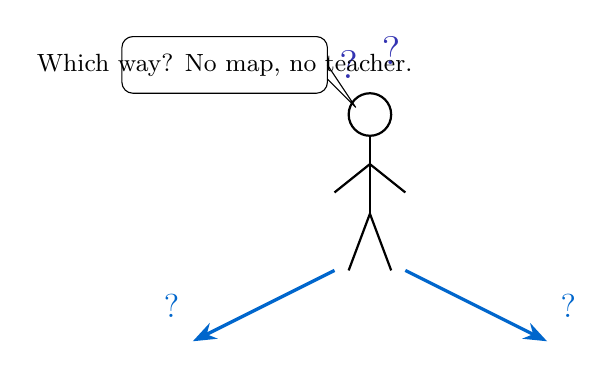
\begin{tikzpicture}[scale=0.9]
% Stick figure at center
\draw[thick] (0,2.2) circle (0.3);
\draw[thick] (0,1.9) -- (0,0.8);
\draw[thick] (0,1.5) -- (-0.5,1.1);
\draw[thick] (0,1.5) -- (0.5,1.1);
\draw[thick] (0,0.8) -- (-0.3,0);
\draw[thick] (0,0.8) -- (0.3,0);
% T-junction arrows
\draw[-{Stealth}, very thick, mlblue] (-0.5,0.0) -- (-2.5,-1.0);
\node[font=\large, mlblue] at (-2.8,-0.5) {?};
\draw[-{Stealth}, very thick, mlblue] (0.5,0.0) -- (2.5,-1.0);
\node[font=\large, mlblue] at (2.8,-0.5) {?};
% Question marks above head
\node[font=\Large, mlpurple] at (-0.3,2.9) {?};
\node[font=\Large, mlpurple] at (0.3,3.1) {?};
% Speech bubble
\draw[fill=white, rounded corners] (-3.5,2.5) rectangle (-0.6,3.3);
\draw (-0.6,2.7) -- (-0.2,2.3) -- (-0.6,2.9);
\node[font=\small] at (-2.05,2.9) {Which way? No map, no teacher.};
\end{tikzpicture}

\vspace{2mm}
The agent must learn from experience alone.
\bottomnote{RL agents start knowing nothing. They learn entirely from feedback.}
\end{frame}

% Slide 5: What Makes RL Different?
\begin{frame}{What Makes RL Different?}
\centering
\small
\begin{tabular}{l c c c}
\toprule
\textbf{Paradigm} & \textbf{Signal} & \textbf{Data} & \textbf{Use Case} \\
\midrule
Supervised & ``Here's the answer'' & Labeled data & Classification, regression \\
Unsupervised & ``Find patterns'' & No labels & Clustering, dim.\ reduction \\
\textbf{RL} & \textbf{``Try and learn''} & \textbf{Rewards/penalties} & \textbf{Decision-making, control} \\
\bottomrule
\end{tabular}

\vspace{5mm}
\highlight{RL is the only paradigm where the agent actively interacts with its environment.}
\bottomnote{RL is the only paradigm where the agent actively interacts with its environment.}
\end{frame}

% Slide 6: CHART --- The RL Loop
\begin{frame}{The Core Idea: Act, Observe, Learn, Repeat}
\centering

\includegraphics[width=0.55\textwidth]{03_rl_loop/chart.pdf}
\begin{compactlist}
\item The agent takes an action in the environment
\item The environment gives back a reward (or penalty)
\item The agent updates its strategy and tries again
\end{compactlist}
\bottomnote{This loop is the foundation of ALL reinforcement learning.}
\end{frame}

% Slide 7: TikZ Comic C2 --- "The Maze Runner"
\begin{frame}{RL: Learning by Trying, Failing, and Trying Again}
\centering
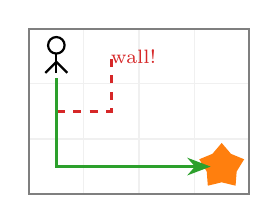
\begin{tikzpicture}[scale=0.7]
% Grid (maze)
\draw[step=1, lightgray] (0,0) grid (4,3);
\draw[mlgray, thick] (0,0) rectangle (4,3);
% Stick figure at start
\draw[thick] (0.5,2.7) circle (0.15);
\draw[thick] (0.5,2.55) -- (0.5,2.2);
\draw[thick] (0.5,2.4) -- (0.3,2.2);
\draw[thick] (0.5,2.4) -- (0.7,2.2);
% Star at goal
\node[star, star points=5, fill=mlorange, minimum size=6mm] at (3.5,0.5) {};
% Wrong path (dashed)
\draw[dashed, mlred, thick] (0.5,2.1) -- (0.5,1.5) -- (1.5,1.5) -- (1.5,2.5);
\node[font=\scriptsize, mlred] at (1.9,2.5) {wall!};
% Learned path (solid)
\draw[mlgreen, very thick, -{Stealth}] (0.5,2.1) -- (0.5,0.5) -- (3.3,0.5);
\end{tikzpicture}

\vspace{2mm}
The agent doesn't know the map --- it learns by exploring.
\bottomnote{Reinforcement Learning = learn from experience, not from labeled examples.}
\end{frame}

% Slide 8: CHART --- Q-Learning Grid
\begin{frame}{Watch the Agent Learn the Best Path}
\centering

\includegraphics[width=0.55\textwidth]{04_q_learning_grid/chart.pdf}
\vspace{-2mm}
\begin{compactlist}
\item Arrows show the agent's best guess for direction
\item After many episodes, arrows converge to the optimal path
\item Discovered by trial and error --- no teacher told it
\end{compactlist}
\bottomnote{Q-learning stores a ``quality'' score for each state-action pair. Higher Q = better action.}
\end{frame}

% Slide 9: How RL Works (No Math)
\begin{frame}{How RL Works (No Math)}
\begin{enumerate}
\setlength{\itemsep}{5pt}
\item \textbf{Try an action} --- the agent does something (move left, buy, sell)

\begin{tikzpicture}[baseline=-0.5ex]
\draw[-{Stealth}, thick, mlblue] (0,0) -- (0.7,0);
\end{tikzpicture}
\item \textbf{Get feedback} --- the environment gives a reward (+1) or penalty ($-$1)

\begin{tikzpicture}[baseline=-0.5ex]
\node[star, star points=5, fill=mlorange, minimum size=4mm] at (0,0) {};
\end{tikzpicture}
\item \textbf{Update strategy} --- remember what worked, avoid what didn't

\begin{tikzpicture}[baseline=-0.5ex]
\draw[thick, mlpurple] (0,0) circle (0.2);
\draw[thick, mlpurple] (-0.15,0.25) -- (-0.05,0.4);
\draw[thick, mlpurple] (0.15,0.25) -- (0.05,0.4);
\draw[thick, mlpurple] (0,0.25) -- (0,0.4);
\end{tikzpicture}
\end{enumerate}
\vspace{3mm}
\begin{block}{The Secret}
Repeat thousands of times. The agent gets better.
\end{block}
\bottomnote{RL agents typically need millions of episodes to learn. That is why simulation is so important.}
\end{frame}

% Slide 10: CHART --- Reward Curves
\begin{frame}{Proof It Works: Rewards Go Up Over Time}
\centering

\includegraphics[width=0.60\textwidth]{05_reward_curves/chart.pdf}
\begin{compactlist}
\item The y-axis shows cumulative reward
\item The line goes up = the agent is getting better
\item Early episodes are random; later episodes show learned behavior
\end{compactlist}
\bottomnote{A rising reward curve is the universal sign of a learning agent.}
\end{frame}

% Slide 11: CHART --- Explore vs Exploit
\begin{frame}{The Key Tradeoff: Explore or Exploit?}
\centering

\includegraphics[width=0.60\textwidth]{top10_09_epsilon_greedy/chart.pdf}
\begin{compactlist}
\item \textbf{Explore} = try something new (might find better)
\item \textbf{Exploit} = stick with what works (safe but might miss better)
\item Epsilon-greedy: explore with probability epsilon, exploit otherwise
\end{compactlist}
\bottomnote{Too much exploration = never settles. Too much exploitation = misses the best strategy.}
\end{frame}

% Slide 12: CHART --- Policy Visualization
\begin{frame}{The End Goal: A Learned Policy}
\centering

\includegraphics[width=0.60\textwidth]{06_policy_viz/chart.pdf}
\begin{compactlist}
\item A policy maps states to actions
\item This is what the agent learned after training
\item The goal is an optimal policy --- best action for every state
\end{compactlist}
\bottomnote{The policy is the agent's strategy --- its complete plan for every situation.}
\end{frame}

% Slide 13: RL Gotchas
\begin{frame}{Three Things to Watch Out For}
\begin{enumerate}
\setlength{\itemsep}{6pt}
\item \textcolor{mlred}{\textbf{!}} \textbf{Needs LOTS of practice} --- millions of episodes. That's why we train in simulation first.
\item \textcolor{mlred}{\textbf{!}} \textbf{Reward design is tricky} --- the agent finds loopholes you didn't expect. Design rewards carefully.
\item \textcolor{mlred}{\textbf{!}} \textbf{Sim-to-real gap} --- what works in simulation may not work in the real world without fine-tuning.
\end{enumerate}
\bottomnote{RL is powerful but hungry: it needs massive compute and careful reward engineering.}
\end{frame}

% Slide 14: Finance Application
\begin{frame}{RL in Finance}
\begin{compactlist}
\item \textbf{Algorithmic trading strategies}: learn when to buy, sell, or hold
\item \textbf{Portfolio rebalancing}: optimize asset allocation over time
\item \textbf{Optimal order execution}: minimize market impact of large trades
\end{compactlist}
\vspace{3mm}
\begin{block}{Bottom Line}
RL excels wherever you need sequential decisions under uncertainty.
\end{block}
\bottomnote{JPMorgan and Two Sigma use RL for trade execution optimization.}
\end{frame}

% Slide 15: Try It Yourself
\begin{frame}{Try It Yourself: The RL Recipe}
\vspace{2mm}
\footnotesize
\texttt{for each episode:}\\[2pt]
\texttt{~~observe state, pick action}\\[2pt]
\texttt{~~get reward, update strategy}\\[2pt]
\texttt{~~repeat until done}

\vspace{5mm}
\normalsize
Start simple: OpenAI Gym provides ready-made environments to practice.
\bottomnote{pip install gymnasium. Try CartPole or FrozenLake as your first RL environment.}
\end{frame}

% Slide 16: TikZ Comic C3 + Key Takeaways
\begin{frame}{The Expert Agent}
\centering
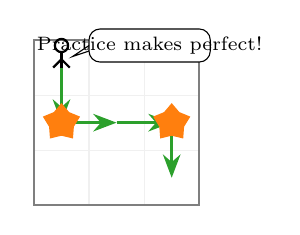
\begin{tikzpicture}[scale=0.7]
% 3x3 grid
\draw[step=1, lightgray] (0,0) grid (3,3);
\draw[mlgray, thick] (0,0) rectangle (3,3);
% Path with green arrows
\draw[mlgreen, very thick, -{Stealth}] (0.5,2.5) -- (0.5,1.5);
\draw[mlgreen, very thick, -{Stealth}] (0.5,1.5) -- (1.5,1.5);
\draw[mlgreen, very thick, -{Stealth}] (1.5,1.5) -- (2.5,1.5);
\draw[mlgreen, very thick, -{Stealth}] (2.5,1.5) -- (2.5,0.5);
% Stars along path
\node[star, star points=5, fill=mlorange, minimum size=4mm] at (0.5,1.5) {};
\node[star, star points=5, fill=mlorange, minimum size=4mm] at (2.5,1.5) {};
% Stick figure walking confidently
\draw[thick] (0.5,2.9) circle (0.12);
\draw[thick] (0.5,2.78) -- (0.5,2.5);
\draw[thick] (0.5,2.65) -- (0.35,2.5);
\draw[thick] (0.5,2.65) -- (0.65,2.5);
% Speech bubble
\draw[fill=white, rounded corners] (1.0,2.6) rectangle (3.2,3.2);
\draw (1.0,2.8) -- (0.7,2.7) -- (1.0,2.9);
\node[font=\scriptsize] at (2.1,2.9) {Practice makes perfect!};
\end{tikzpicture}

\vspace{2mm}
\begin{enumerate}
\setlength{\itemsep}{3pt}
\item RL agents learn by trial and error with rewards
\item Explore vs exploit is the key tradeoff
\item Finance uses: trading, portfolio optimization, order execution
\end{enumerate}
\bottomnote{RL: learning to make better decisions, one episode at a time.}
\end{frame}

% Slide 17: XKCD Closing
\begin{frame}{Go Teach a Machine Something}
\centering
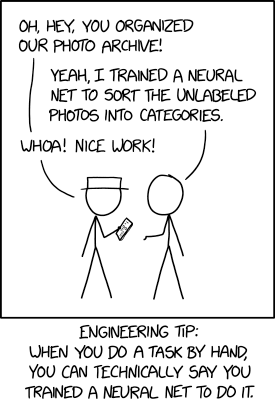
\includegraphics[height=0.55\textheight]{images/2173_trained_a_neural_net.png}
\bottomnote{XKCD \#2173 by Randall Munroe (CC BY-NC 2.5). Next: try the Jupyter notebook to train your own RL agent!}
\end{frame}

\end{document}
